\documentclass{beamer}
\useoutertheme[progressbar=frametitle]{metropolis}
\useinnertheme{metropolis}
\definecolor{nabgray}{rgb}{0.6,0.59,0.61}
\usecolortheme[named=nabgray]{structure}
\usepackage{tikz}
\usepackage[utf8]{inputenc}
\usepackage[spanish]{babel}

\usepackage{smartdiagram}
\usepackage{qtree}
\usepackage{verbatim}
\usepackage{svg}
\usepackage{graphicx}
\usepackage{color}
\definecolor{lightgray}{rgb}{0.95, 0.95, 0.95}
\definecolor{darkgray}{rgb}{0.4, 0.4, 0.4}
%\definecolor{purple}{rgb}{0.65, 0.12, 0.82}
\definecolor{editorGray}{rgb}{0.95, 0.95, 0.95}
\definecolor{editorOcher}{rgb}{1, 0.5, 0} % #FF7F00 -> rgb(239, 169, 0)
\definecolor{editorGreen}{rgb}{0, 0.5, 0} % #007C00 -> rgb(0, 124, 0)
\definecolor{orange}{rgb}{1,0.45,0.13}		
\definecolor{olive}{rgb}{0.17,0.59,0.20}
\definecolor{brown}{rgb}{0.69,0.31,0.31}
\definecolor{purple}{rgb}{0.38,0.18,0.81}
\definecolor{lightblue}{rgb}{0.1,0.57,0.7}
\definecolor{lightred}{rgb}{1,0.4,0.5}
\usepackage{upquote}
\usepackage{listings}
\lstset{language=java,
	basicstyle=\footnotesize\ttfamily,
	keywordstyle=\footnotesize\color{blue}\ttfamily,
}


\usebackgroundtemplate
{
	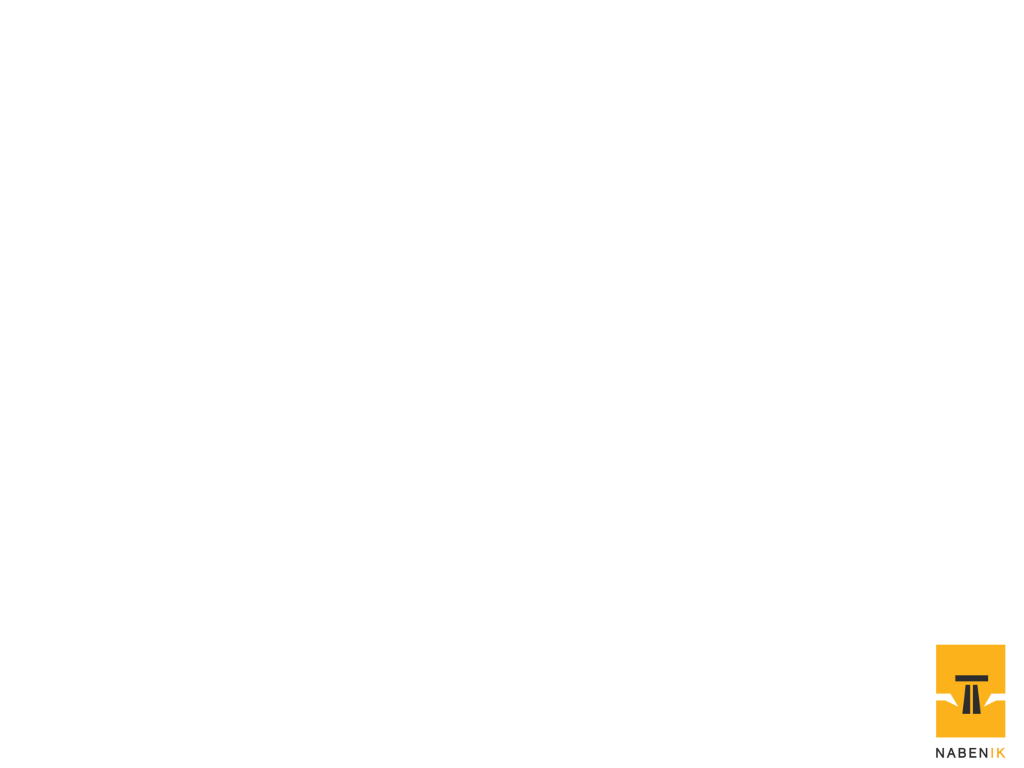
\includegraphics[width=\paperwidth]{Images/fondo}%
}


\title{Principios de GC para JVM y Android}
\author{Víctor Orozco - @tuxtor}
\institute{GuateJUG}
\date{\today}

\begin{document}

\frame{\titlepage}


\section{¿Porque Java?}
\begin{frame}
\huge ¿Porque Java?
\end{frame}

\begin{frame}
JAVA IS DEAD
\begin{figure}
\centering
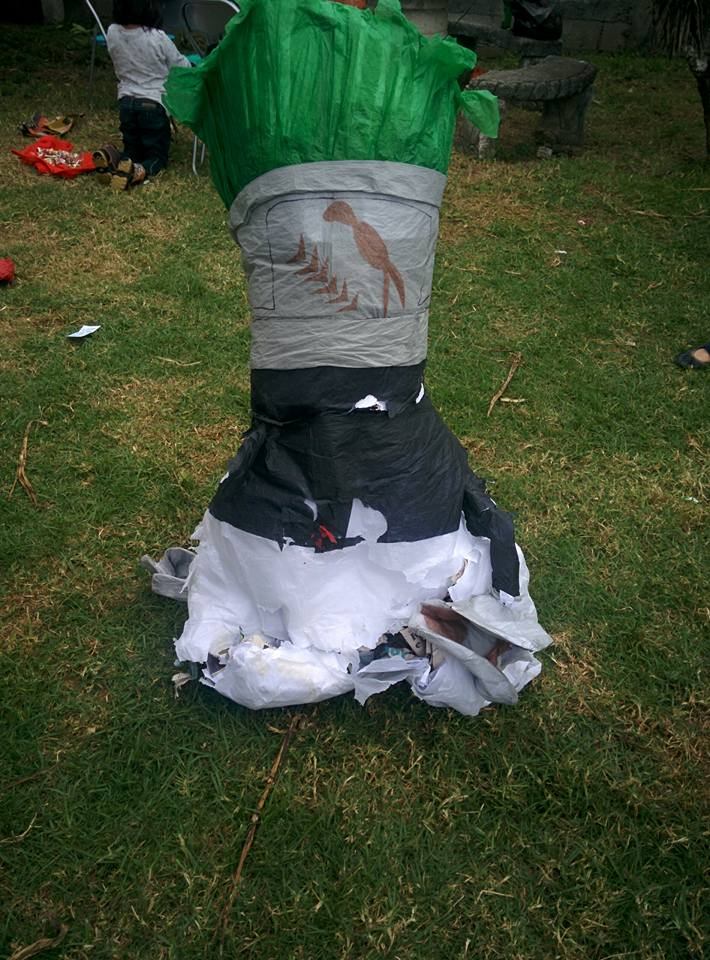
\includegraphics[width=0.5\linewidth]{Images/dukedead.jpg}
\end{figure}
\end{frame}

\begin{frame}
\begin{figure}
\centering

\includegraphics[width=0.5\linewidth]{Images/javadead}
\end{figure}
\end{frame}

\begin{frame}
\begin{figure}
\centering
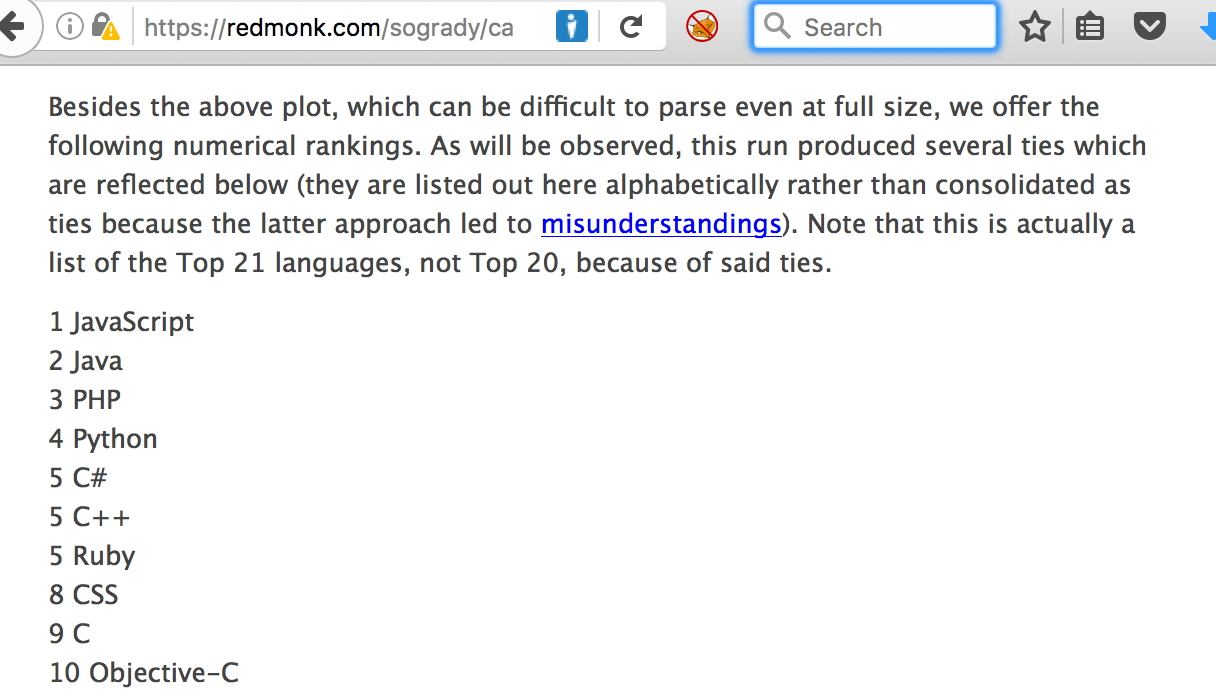
\includegraphics[width=0.9\linewidth]{Images/redmonk}
\end{figure}
\end{frame}

\begin{frame}
\begin{figure}
\centering
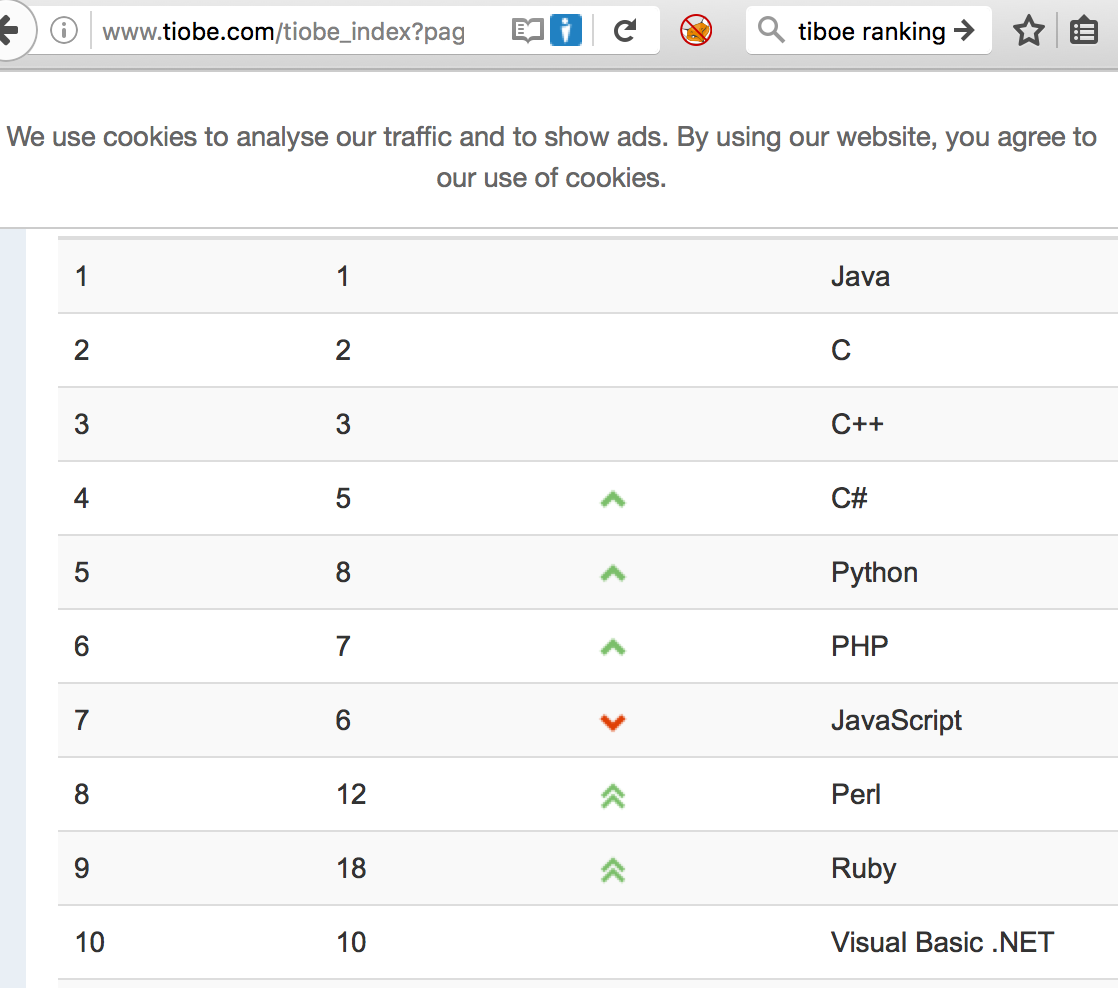
\includegraphics[width=0.9\linewidth]{Images/tiboe}
\end{figure}
\end{frame}

\section{Java}
\begin{frame}
\huge ¿Que es Java?
\end{frame}

\begin{frame}{Lenguaje}
\begin{figure}
\centering
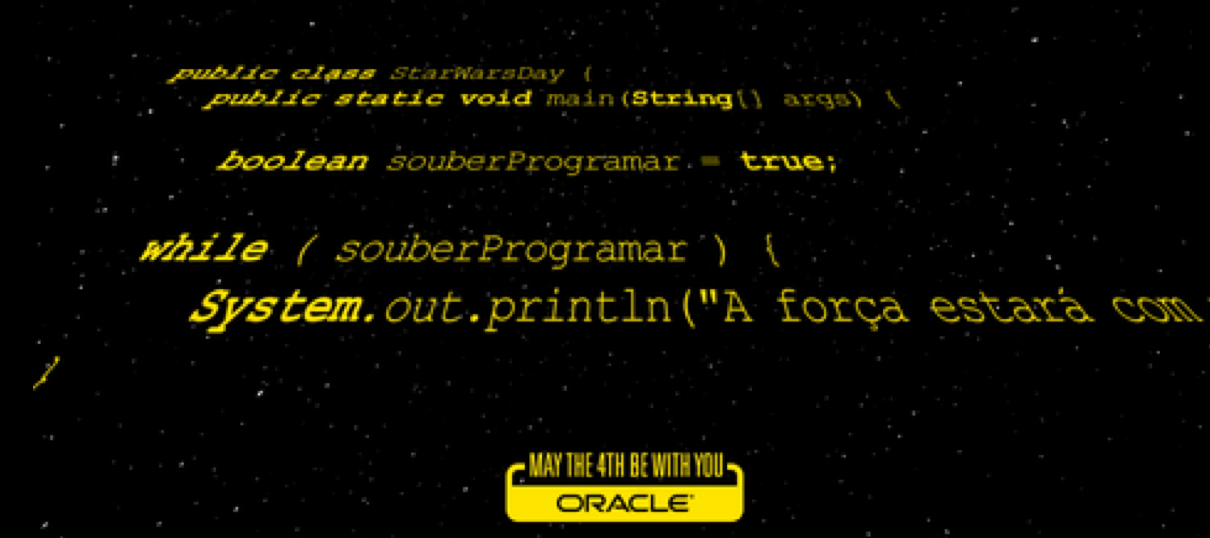
\includegraphics[width=0.9\linewidth]{Images/javalang}
\end{figure}
\end{frame}

\begin{frame}{Maquina virtual}
\begin{figure}
\centering
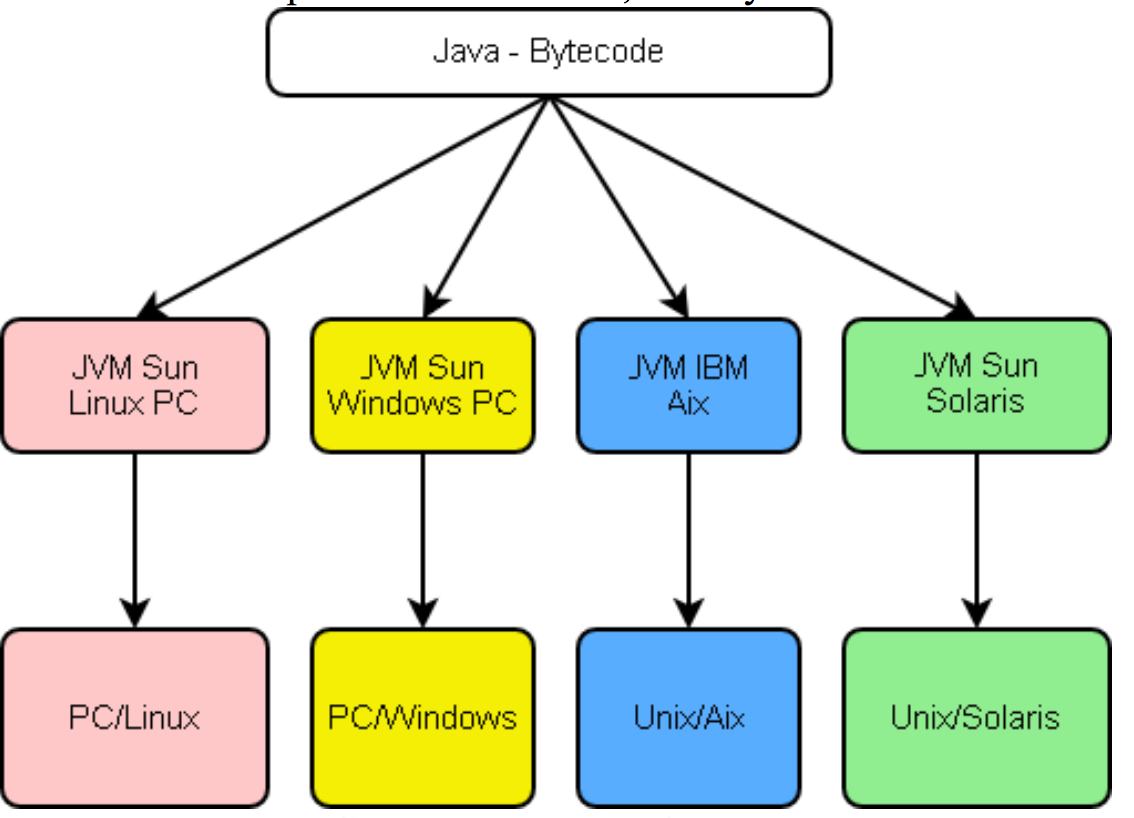
\includegraphics[width=0.9\linewidth]{Images/jvm}
\end{figure}
\end{frame}

\begin{frame}{Muchas plataformas}
\begin{figure}
\centering
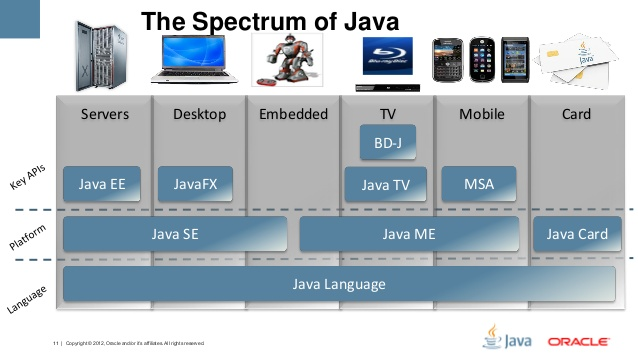
\includegraphics[width=0.9\linewidth]{Images/spectrum}
\end{figure}
\end{frame}


\begin{frame}{GC}
\Large ¿CMS? ¿Stack heap? ¿GC Generacional? ¿Porqué mis aplicaciones explotan y Facebook no?
\begin{figure}
	\centering
	
\includegraphics[width=0.6\linewidth]{Images/dukewhy}
\end{figure}
\end{frame}


\begin{frame}{TLDR}
Explosión
\begin{itemize}
	\item Mala selección de tipos de dato
	\item Muchas variables y referencias (memory leak)
	\item Algoritmos innecesariamente complejos
	\item Muchas apps y poca memoria
\end{itemize}

\end{frame}

\section{Memoria en VMs}
\begin{frame}{Stack vs heap}
\begin{figure}
	\centering
	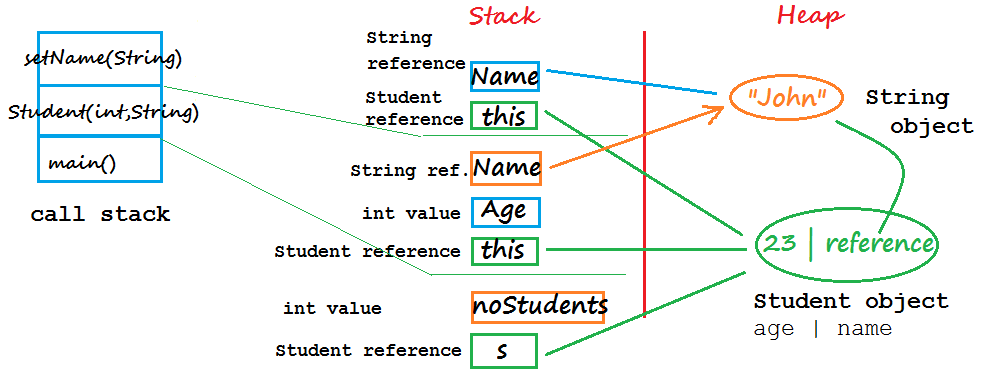
\includegraphics[width=\linewidth]{Images/heap}
	\caption{Stack y Heap}
	\label{fig:heap}
\end{figure}

\end{frame}

\begin{frame}{Stack vs heap}
\begin{figure}
	\centering
	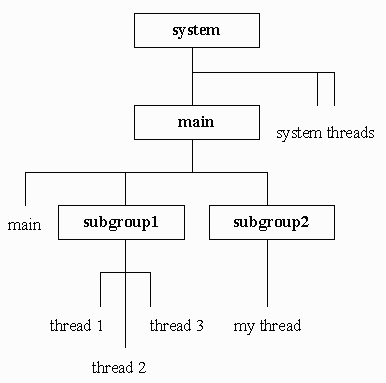
\includegraphics[width=0.6\linewidth]{Images/jthreads}
	\caption{Java main thread}
	\label{fig:jthreads}
\end{figure}

\end{frame}

\begin{frame}{Mark and sweep}
\begin{figure}
	\centering
	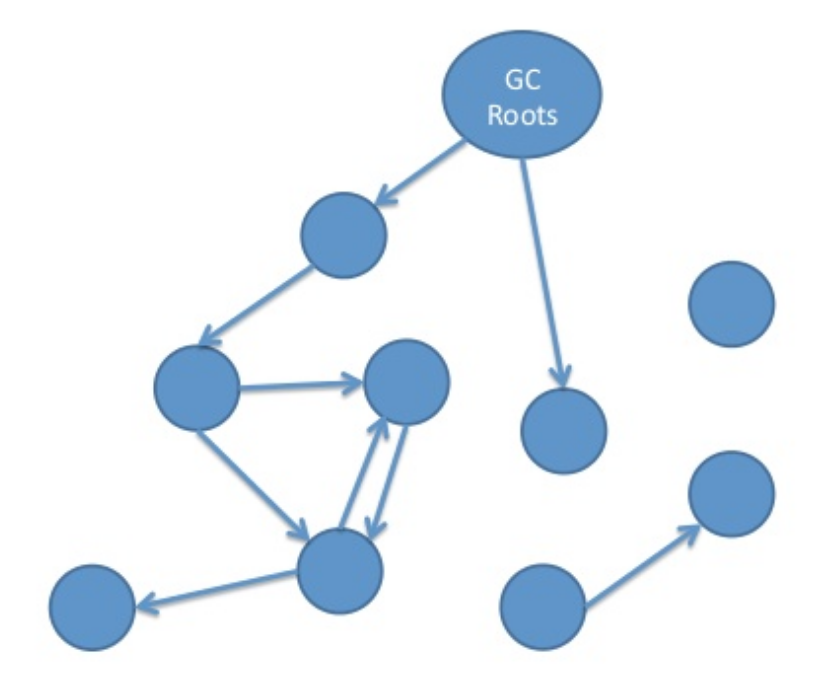
\includegraphics[width=0.6\linewidth]{Images/gc1}
	\caption{Mark and sweep, Credits: https://plumbr.io}
	\label{fig:markandsweep}
\end{figure}
\end{frame}

\begin{frame}{Mark and sweep}
\begin{figure}
	\centering
	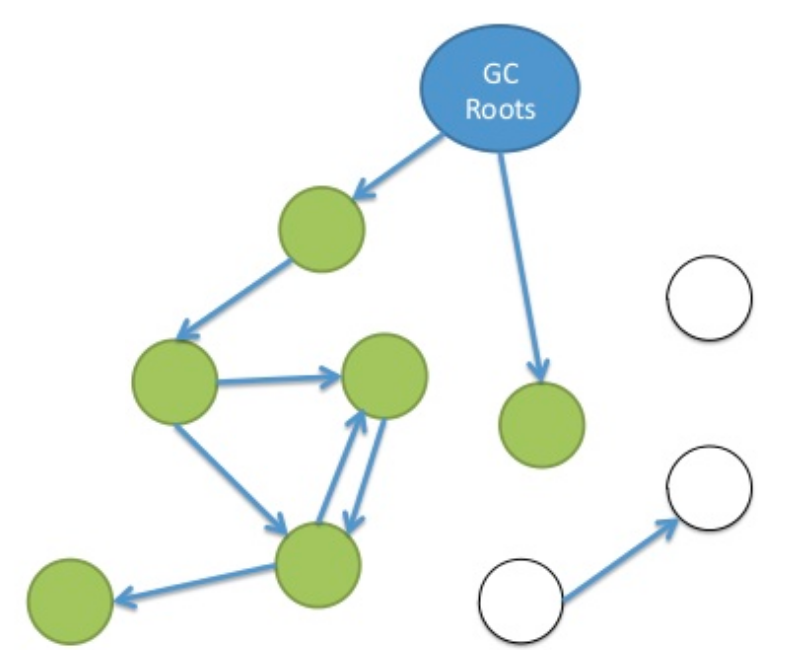
\includegraphics[width=0.6\linewidth]{Images/gc2}
	\caption{Mark and sweep - Mark, Credits: https://plumbr.io}
	\label{fig:mark}
\end{figure}
Generalmente DFS
\end{frame}

\begin{frame}{Mark and sweep}
\begin{figure}
	\centering
	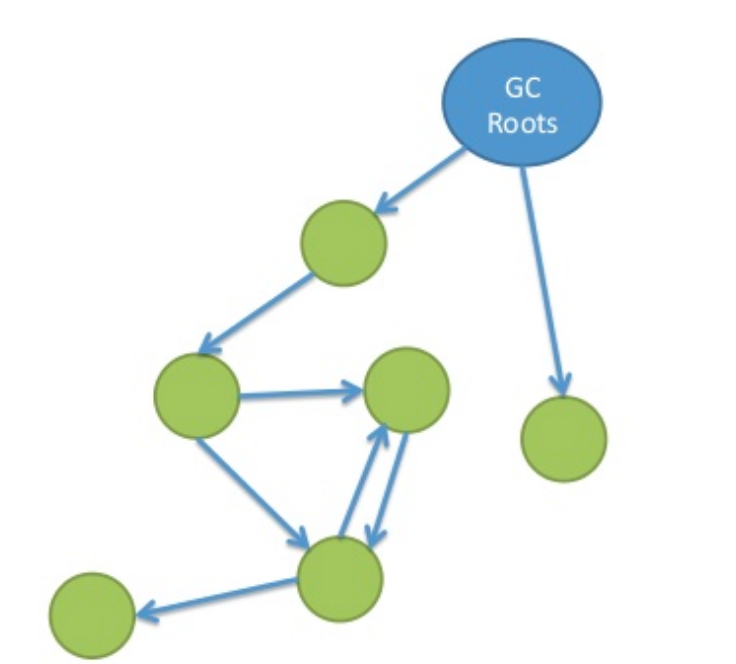
\includegraphics[width=0.6\linewidth]{Images/gc3}
	\caption{Mark and sweep - sweep, Credits: https://plumbr.io}
	\label{fig:sweep}
\end{figure}
\end{frame}

\begin{frame}{Mark and sweep}
\begin{figure}
	\centering
	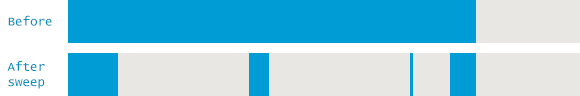
\includegraphics[width=\linewidth]{Images/gcsweep}
	\caption{Mark - sweep, Credits: https://plumbr.io}
	\label{fig:sweeporig}
\end{figure}
\end{frame}

\begin{frame}{Mark - sweep - compact}
\begin{figure}
	\centering
	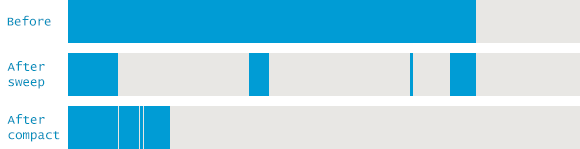
\includegraphics[width=\linewidth]{Images/gccompact}
	\caption{Mark - sweep - compact, Credits: https://plumbr.io}
	\label{fig:sweepcompact}
\end{figure}
\end{frame}

\begin{frame}{Mark and copy}
\begin{figure}
	\centering
	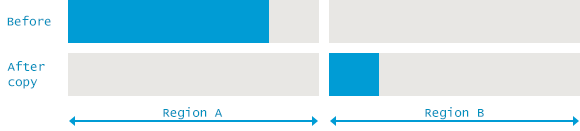
\includegraphics[width=\linewidth]{Images/gccopy}
	\caption{Mark and copy, Credits: https://plumbr.io}
	\label{fig:sweepcopy}
\end{figure}
\end{frame}

\begin{frame}[fragile]{Demo 0 - Generación de objetos}
\begin{lstlisting}
//...
Stream<Integer> nums = Stream.iterate(1, n -> n + 1);

nums.forEach(num -> {
		System.out.println(num);
		try{Thread.sleep(10);}
		catch(InterruptedException ex){}
	}
);
//...
\end{lstlisting}
\end{frame}

\section{Generational garbage collectors}

\begin{frame}{Generational GC(HotSpot)}
\begin{figure}
	\centering
	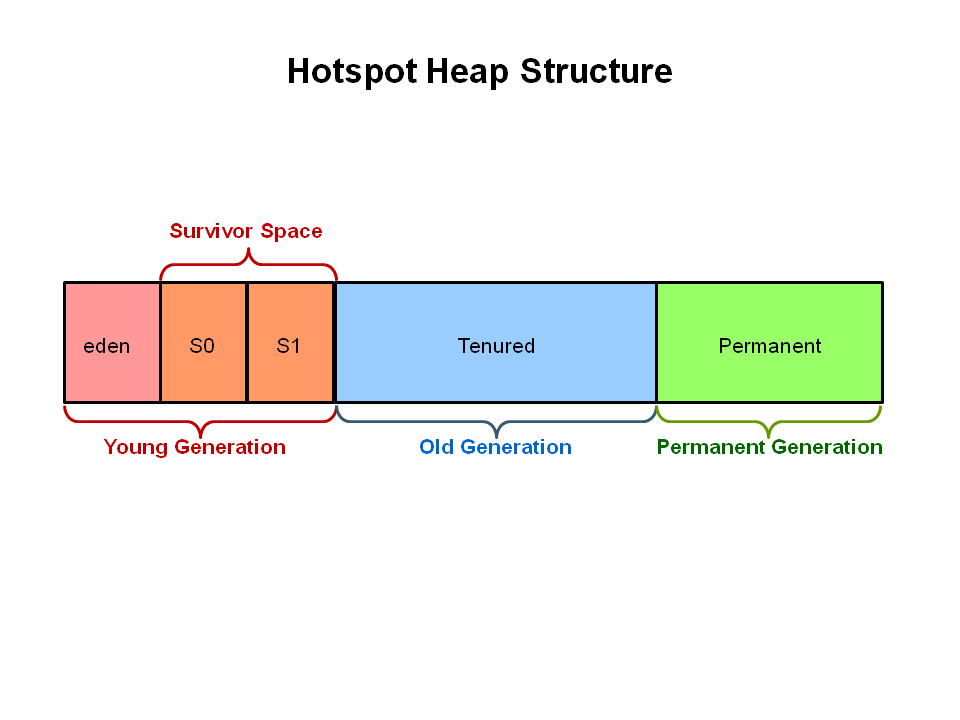
\includegraphics[width=0.9\linewidth]{Images/generational}
	\caption{Generational GC, Credits: Oracle}
\end{figure}
\end{frame}

\begin{frame}{Generational GC(HotSpot)}
\begin{figure}
	\centering
	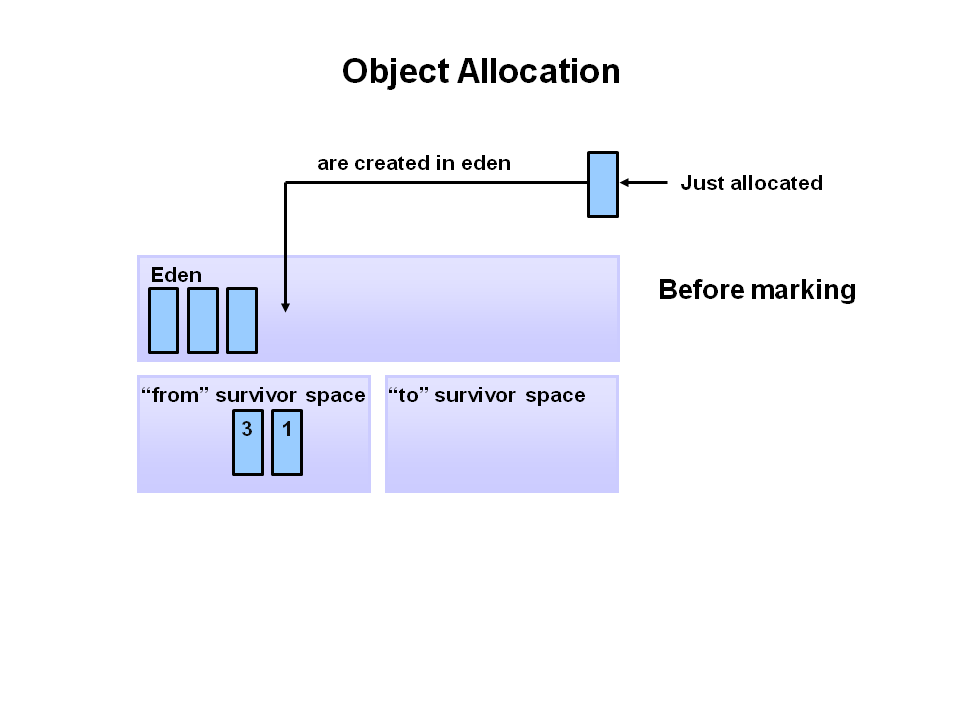
\includegraphics[width=0.9\linewidth]{Images/generational1}
	\caption{Generational GC, Credits: Oracle}
\end{figure}
\end{frame}

\begin{frame}{Generational GC(HotSpot)}
\begin{figure}
	\centering
	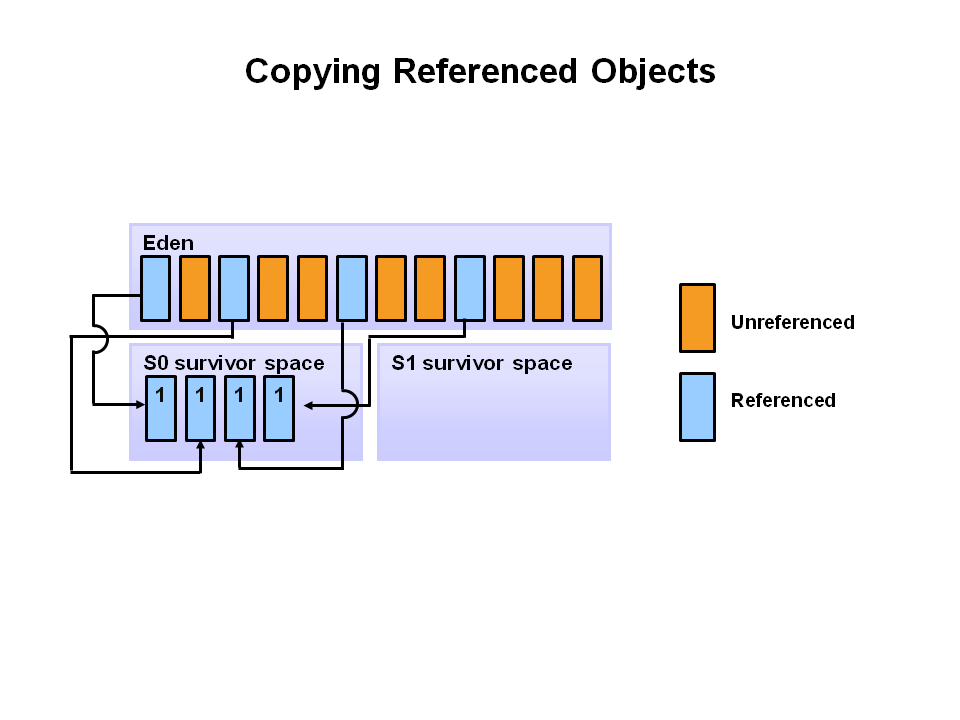
\includegraphics[width=0.9\linewidth]{Images/generational2}
	\caption{Generational GC, Credits: Oracle}
\end{figure}
\end{frame}

\begin{frame}{Generational GC(HotSpot)}
\begin{figure}
	\centering
	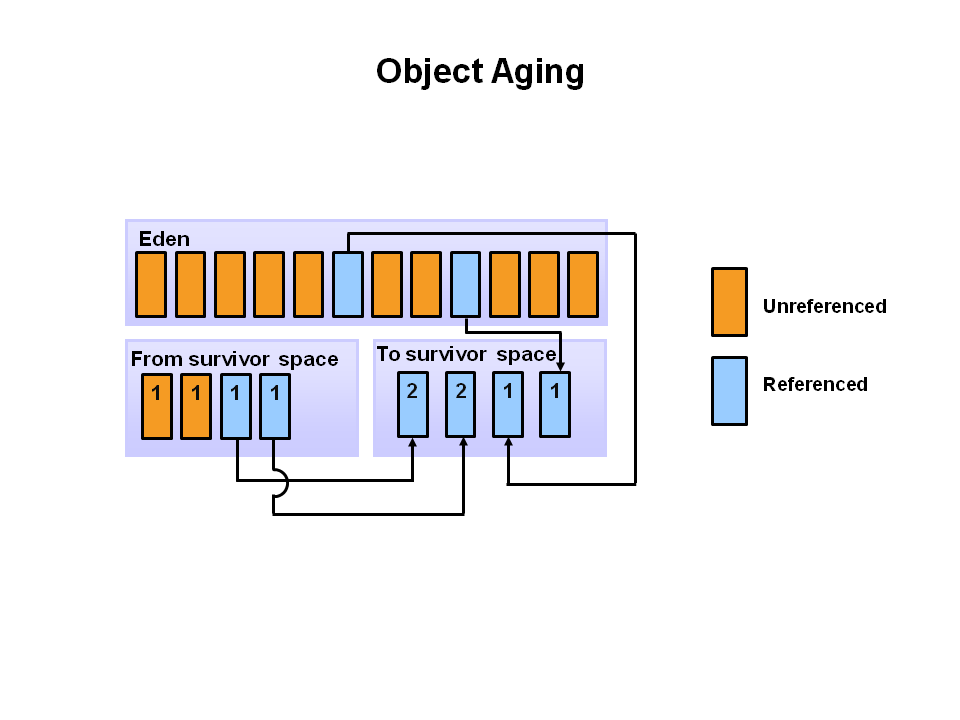
\includegraphics[width=0.9\linewidth]{Images/generational3}
	\caption{Generational GC, Credits: Oracle}
\end{figure}
\end{frame}

\begin{frame}{Generational GC(HotSpot)}
\begin{figure}
	\centering
	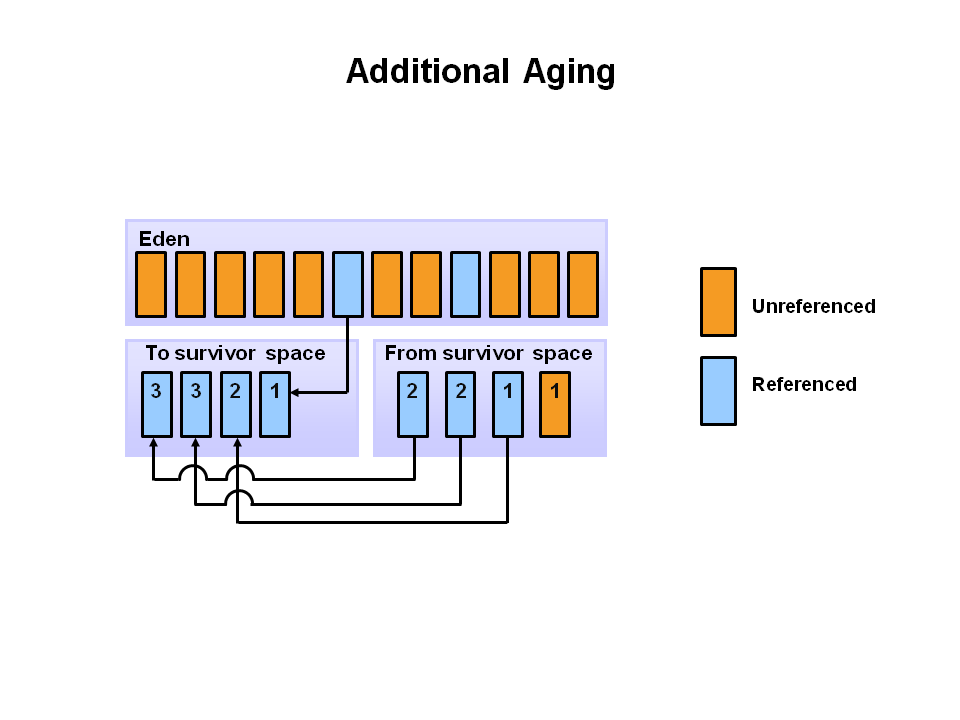
\includegraphics[width=0.9\linewidth]{Images/generational4}
	\caption{Generational GC, Credits: Oracle}
\end{figure}
\end{frame}

\begin{frame}{Generational GC(HotSpot)}
\begin{figure}
	\centering
	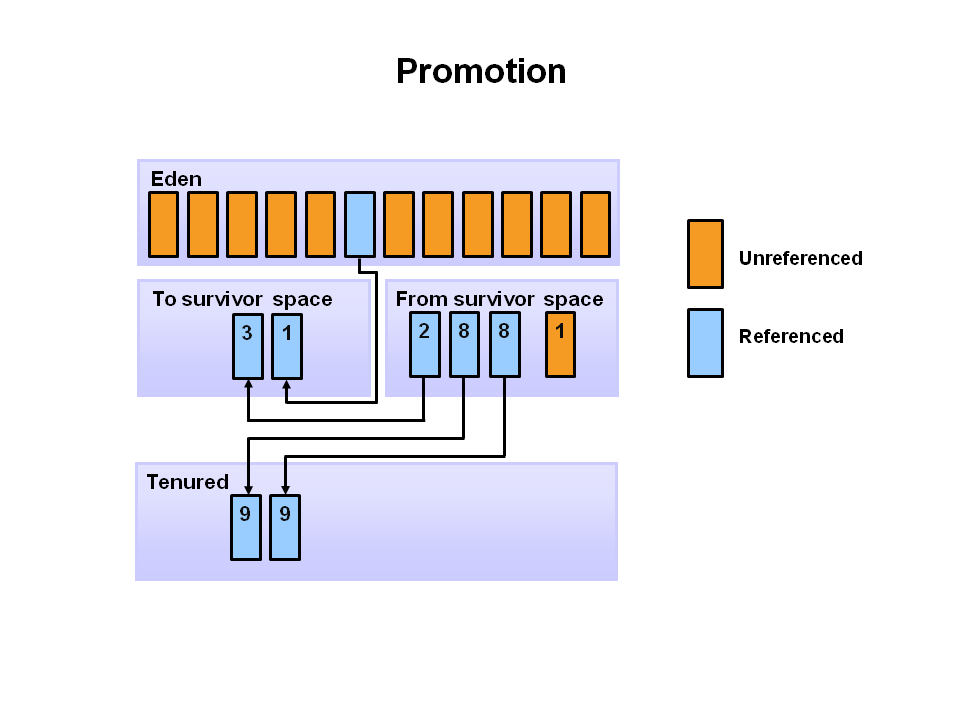
\includegraphics[width=0.9\linewidth]{Images/generational5}
	\caption{Generational GC, Credits: Oracle}
\end{figure}
\end{frame}

\begin{frame}{Generational GC(HotSpot)}
\begin{figure}
	\centering
	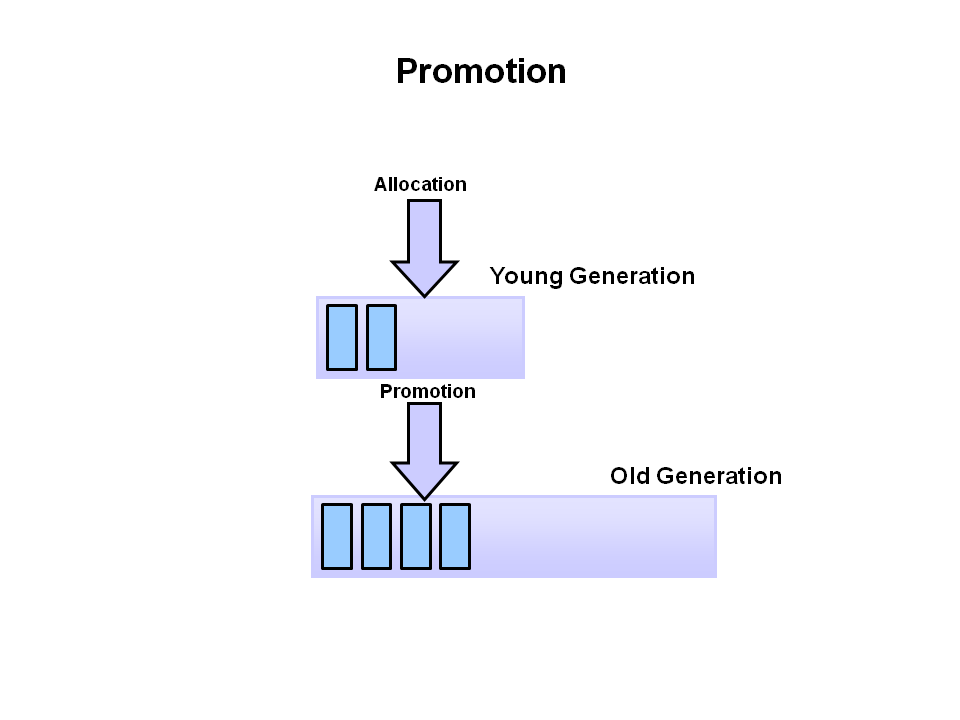
\includegraphics[width=0.9\linewidth]{Images/generational6}
	\caption{Generational GC, Credits: Oracle}
\end{figure}
\end{frame}

\begin{frame}[fragile]{Demo 1 - GC Generacional}
\begin{lstlisting}
//...
Stream<Integer> nums = Stream.iterate(1, n -> n + 1);

var numeros = new ArrayList<Integer>();

nums.forEach(num -> {
	System.out.println(num);
	numeros.add(num);
});
//...
\end{lstlisting}
\begin{quote}
	java -XX:+UseSerialGC GenerationsDemo
\end{quote}
\end{frame}

\section{GC en OpenJDK y Android}
\begin{frame}[fragile]{Recolectores de basura}
OpenJDK
\begin{itemize}
	\item Serial GC para Young y Old generations
	\item Parallel GC para Young y Old generations
	\item Parallel New para Young + Concurrent Mark and Sweep (CMS) para Old Generation
	\item G1GC, para Young y Old generations	
\end{itemize}

Android
\begin{itemize}
	\item Sticky CMS
	\item Partial CMS
	\item Full CMS
	\item RosAlloc (Slots Allocator)
\end{itemize}

Tip: Ustedes no controlan la ejecución del GC, solo los OEM
\end{frame}

\begin{frame}[fragile]{SerialGC}
\begin{itemize}
	\item Young: Mark-Copy
	\item Old: Mark-Sweep-Compact
	\item $java -XX:+UseSerialGC com.nabenik.MyExecClass$
\end{itemize}
\end{frame}

\begin{frame}[fragile]{ParallelGC}
\begin{itemize}
	\item Young: Mark-Copy
	\item Old: Mark-Sweep-Compact
	\item Stop-the-world en ambas regiones
	\item $java -XX:+UseParallelGC com.nabenik.MyExecClass$
\end{itemize}
\end{frame}

\begin{frame}[fragile]{CMS}
\begin{itemize}
	\item Young: Mark-Copy - Stop the world
	\item Old: (Mostly )Concurrent Mark Sweep (Paralelo)
	\item $java -XX:+UseConcMarkSweepGC com.nabenik.MyExecClass$
\end{itemize}
\end{frame}

\begin{frame}[fragile]{ART - CMS}
\begin{itemize}
	\item Sticky CMS (non-moving)
	\item Compact = Imperceptible (background/cached )
	\item Young es reemplazado por Allocation Stack (java.lang.Object)
	\item Activity Manager
\end{itemize}
\end{frame}


\begin{frame}[fragile]{ART - CMS}
Explosión
\begin{itemize}
	\item Broadcast Receiver 10 segundos 
	\item Activity Manager 5 segundos
\end{itemize}

\begin{figure}
	\centering
	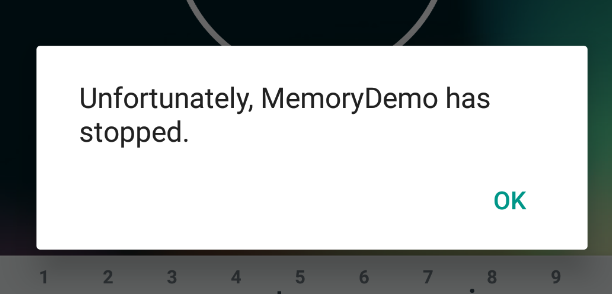
\includegraphics[width=0.7\linewidth]{Images/explosion}
	\caption{Dialogo ANR}
\end{figure}

\end{frame}

\begin{frame}[fragile]{ART - CMS}
\begin{lstlisting}
<application
...
android:largeHeap="true"
...
</application>
\end{lstlisting}
\end{frame}

\section{Como luchar CONTRA un Garbage Collector}

\begin{frame}[fragile]{Demo 1 - Referencias + Mal tipo de dato}
\begin{lstlisting}
//...
var lasReferencias = new ArrayList<String>();
Stream<Integer> numeros = Stream.iterate(1, n -> ++n);

numeros.forEach(n -> {
		lasReferencias.add(n + "");
		if(lasReferencias.size() % 10_000_000 == 0){
		System.out.println(n);
		try{ Thread.sleep(3000); }
		catch(InterruptedException e){}
		}
	});
}
//...
\end{lstlisting}
\end{frame}


\begin{frame}[fragile]{Demo 2 - Referencias}
\begin{lstlisting}
//...
var lasReferencias = new ArrayList<Integer>();
var numeros = IntStream.iterate(1, n -> ++n);

numeros.forEach(n -> {
		lasReferencias.add(n);
		if(lasReferencias.size() % 10_000_000 == 0){
		System.out.println(n);
		try{ Thread.sleep(3000); }
		catch(InterruptedException e){}
	}
});
//...
\end{lstlisting}
\end{frame}

\begin{frame}[fragile]{Demo 3 - Concatenación de String}
\begin{lstlisting}
//...
static String texto = "";
public static void main(String[] args){
	var numeros = IntStream.iterate(1, t -> ++t);
	
	numeros.forEach(n -> {
		texto += " " + n;
		if(n % 10_000 == 0) System.out.println(n);
	});
}
//...
\end{lstlisting}
\end{frame}

\begin{frame}[fragile]{Demo 4 - StringBuffer}
\begin{lstlisting}
//...
static StringBuilder texto = new StringBuilder("");
public static void main(String[] args){
	var numeros = IntStream.iterate(1, t -> ++t);
	
	numeros.forEach(n -> {
		texto.append(" ");
		texto.append(n);
		if(n % 10_000 == 0) System.out.println(n);
	});
}

//...
\end{lstlisting}
\end{frame}

\section{Complejidad de algoritmos}
\begin{frame}{Complejidad}
Complejidad = Cantidad de pasos para realizar una tarea\\
\begin{figure}
	\centering
	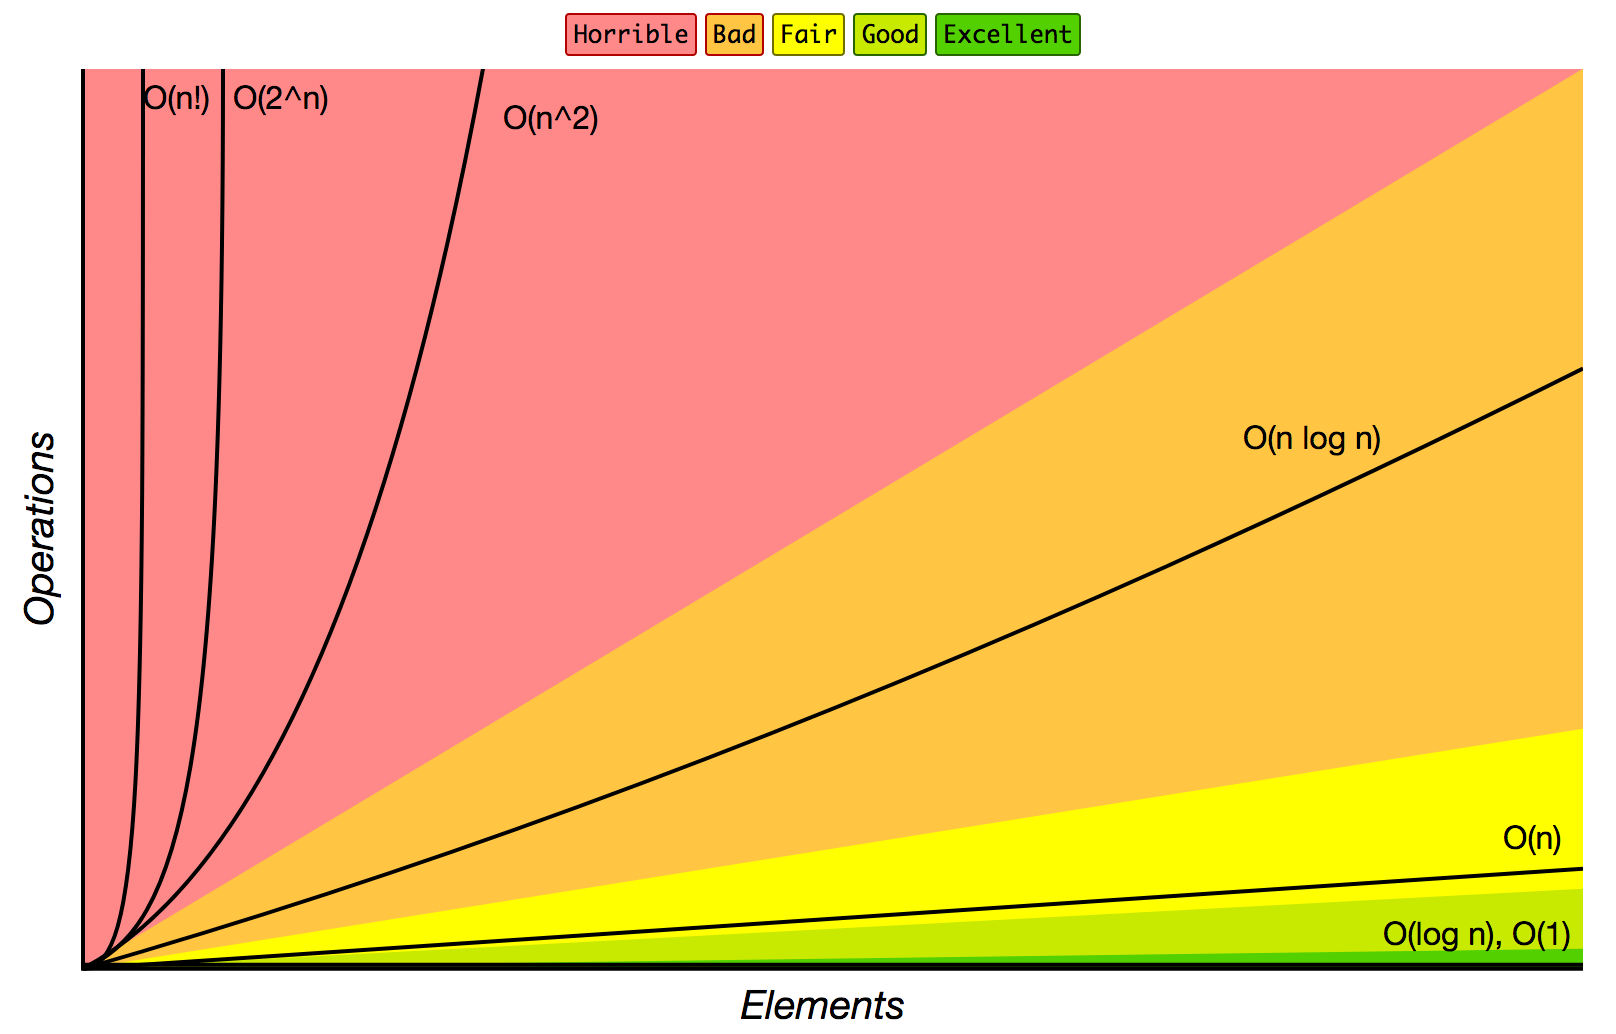
\includegraphics[width=0.7\linewidth]{Images/complex}
	\caption{Complejidad computacional}
	\label{fig:complex}
\end{figure}
También conocido como "programar bien" :O
\end{frame}

\begin{frame}{Fibonacci}
\begin{figure}
	\centering
	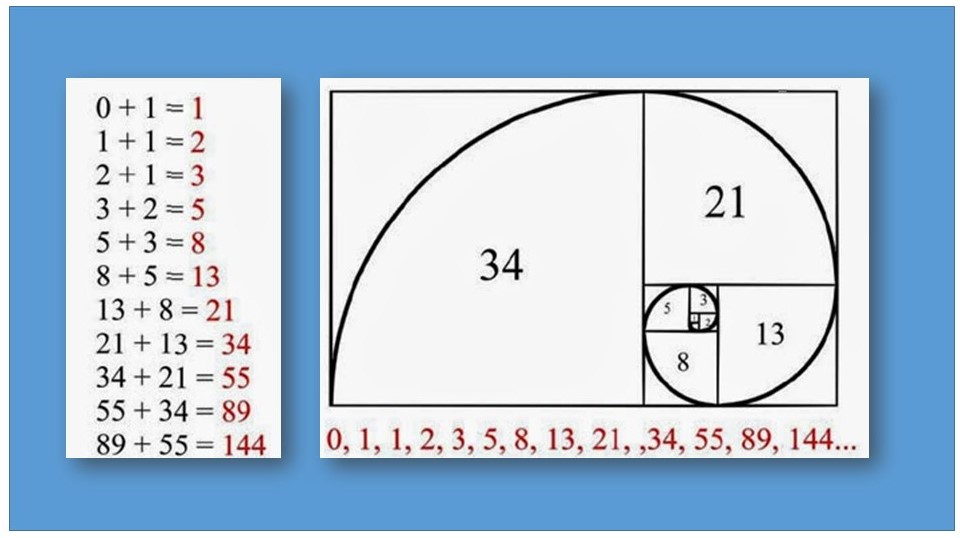
\includegraphics[width=0.7\linewidth]{Images/fibonacci}
	\caption{Sucesión Fibonacci}
	\label{fig:fibonacci}
\end{figure}
\end{frame}

\begin{frame}[fragile]{Demo 5 - Mal Fibonacci}
\begin{lstlisting}
//...
public static long doFibonacci(int n) {
	if (n <= 1)
		return n;
	else
		return doFibonacci(n-1) + doFibonacci(n-2);
}
//...
\end{lstlisting}
\end{frame}

\begin{frame}[fragile]{Demo 6 - Buen Fibonacci}
\begin{lstlisting}
//...
public static long doFibonacci(int n) {
	long a=0, b=1, c=0;
	
	for(int i = 0 ; i < n; i++){
		c = a + b;
		a = b;
		b = c;
	}
	return c;
}
//...
\end{lstlisting}
\end{frame}

\begin{frame}{Víctor Orozco}
\begin{columns}[T] % contents are top vertically aligned
	
	\begin{column}[T]{4cm} % alternative top-align that's better for graphics
		\begin{figure}
			\centering
			
\includegraphics[width=\linewidth]{Images/logos}
		\end{figure}
	\end{column}
	\begin{column}[T]{6cm} % each column can also be its own environment
		\begin{itemize}
			\item me@vorozco.com
			\item \href{https://twitter.com/tuxtor}{@tuxtor}
			\item \href{http://vorozco.com}{http://vorozco.com}
			\item \href{http://tuxtor.shekalug.org}{http://tuxtor.shekalug.org} 
		\end{itemize}
		\begin{center}
			
\includegraphics[width=0.1\linewidth]{Images/cclogo}
			\\
			This work is licensed under a Creative Commons Attribution-ShareAlike 3.0.
		\end{center}
	\end{column}
\end{columns}
\end{frame}

\end{document}

